\todo{Allmän källhänvissning krävs härnere}

\todo{Also graphs are far from final, that font needs to be changed Im jusut really lazy}

%Over the course of this report we have refered to, and approximated, the distribution of variouss classifications of prime numbers. Using now our implementation of Helfgott's origianl code we seek to present the legitimacy of said distributions and also reflect on the quality of the code which we have written. The specific distributions to be presented are those of the regular prime numbers, the twin primes, and a the frequency of various prime gaps will also be presented. For each of these implementations have slight modifications been made to the code, which will be briefly discussed.

Genom rapportens gång har vi hänvisat till, och uppskattat fördelningen av, ett antal klasser av primtal och deras egenskaper. 
Nu, med användning av vår implementering av Helfgotts ursprunglig kod, ämnar vi att först redovisa legitimiteten av vår kod med stöd av primtalssatsens förväntad primtalsfördelning. 
Sedan undersöker vi den möjliga sanningen av en hypotetisk fördelning för tvillingsprimtal. 
Slutligen redovisas frekvensen av primtalsgapp, och mönster som uppträder där i.
För varje implementering vilket kräver justering av koden, kommer dessa modifikationer förklaras kort, därmed finns fullständigt kod för modifikationerna finns med i Appendix XXX - YYY.

\subsubsection{Fördelningen av primtal}\label{app.primes.title}
%Beginning with the classic example of the set of prime numbers, below is illustrated the distribution predicted by the familiar x over log x from sieve theory/Chebychev, the more accurate lorgarithmic integral Li(x), and the actual number of primes found in using our implementation. In order to generate the following graph, no new sieving methods were introduced, simply the counting fucntion in Appendix X

Vi börjar med att jämföra antalet primtal hittat med \textsc{NewSegSiev} emot fördelningen som ges av primtalssatsen, nämligen
\begin{equation}
    \pi(x) \sim Li(x) = \int_2^x\frac{1}{\log t}dt\label{app.primes.PNT}.
\end{equation}
För att skapa följande figur använder vi bara vår implementering av Helfgotts kod och en enkel räknesfunktion, Appendix XXX.

\begin{figure}[H]
    \centering
    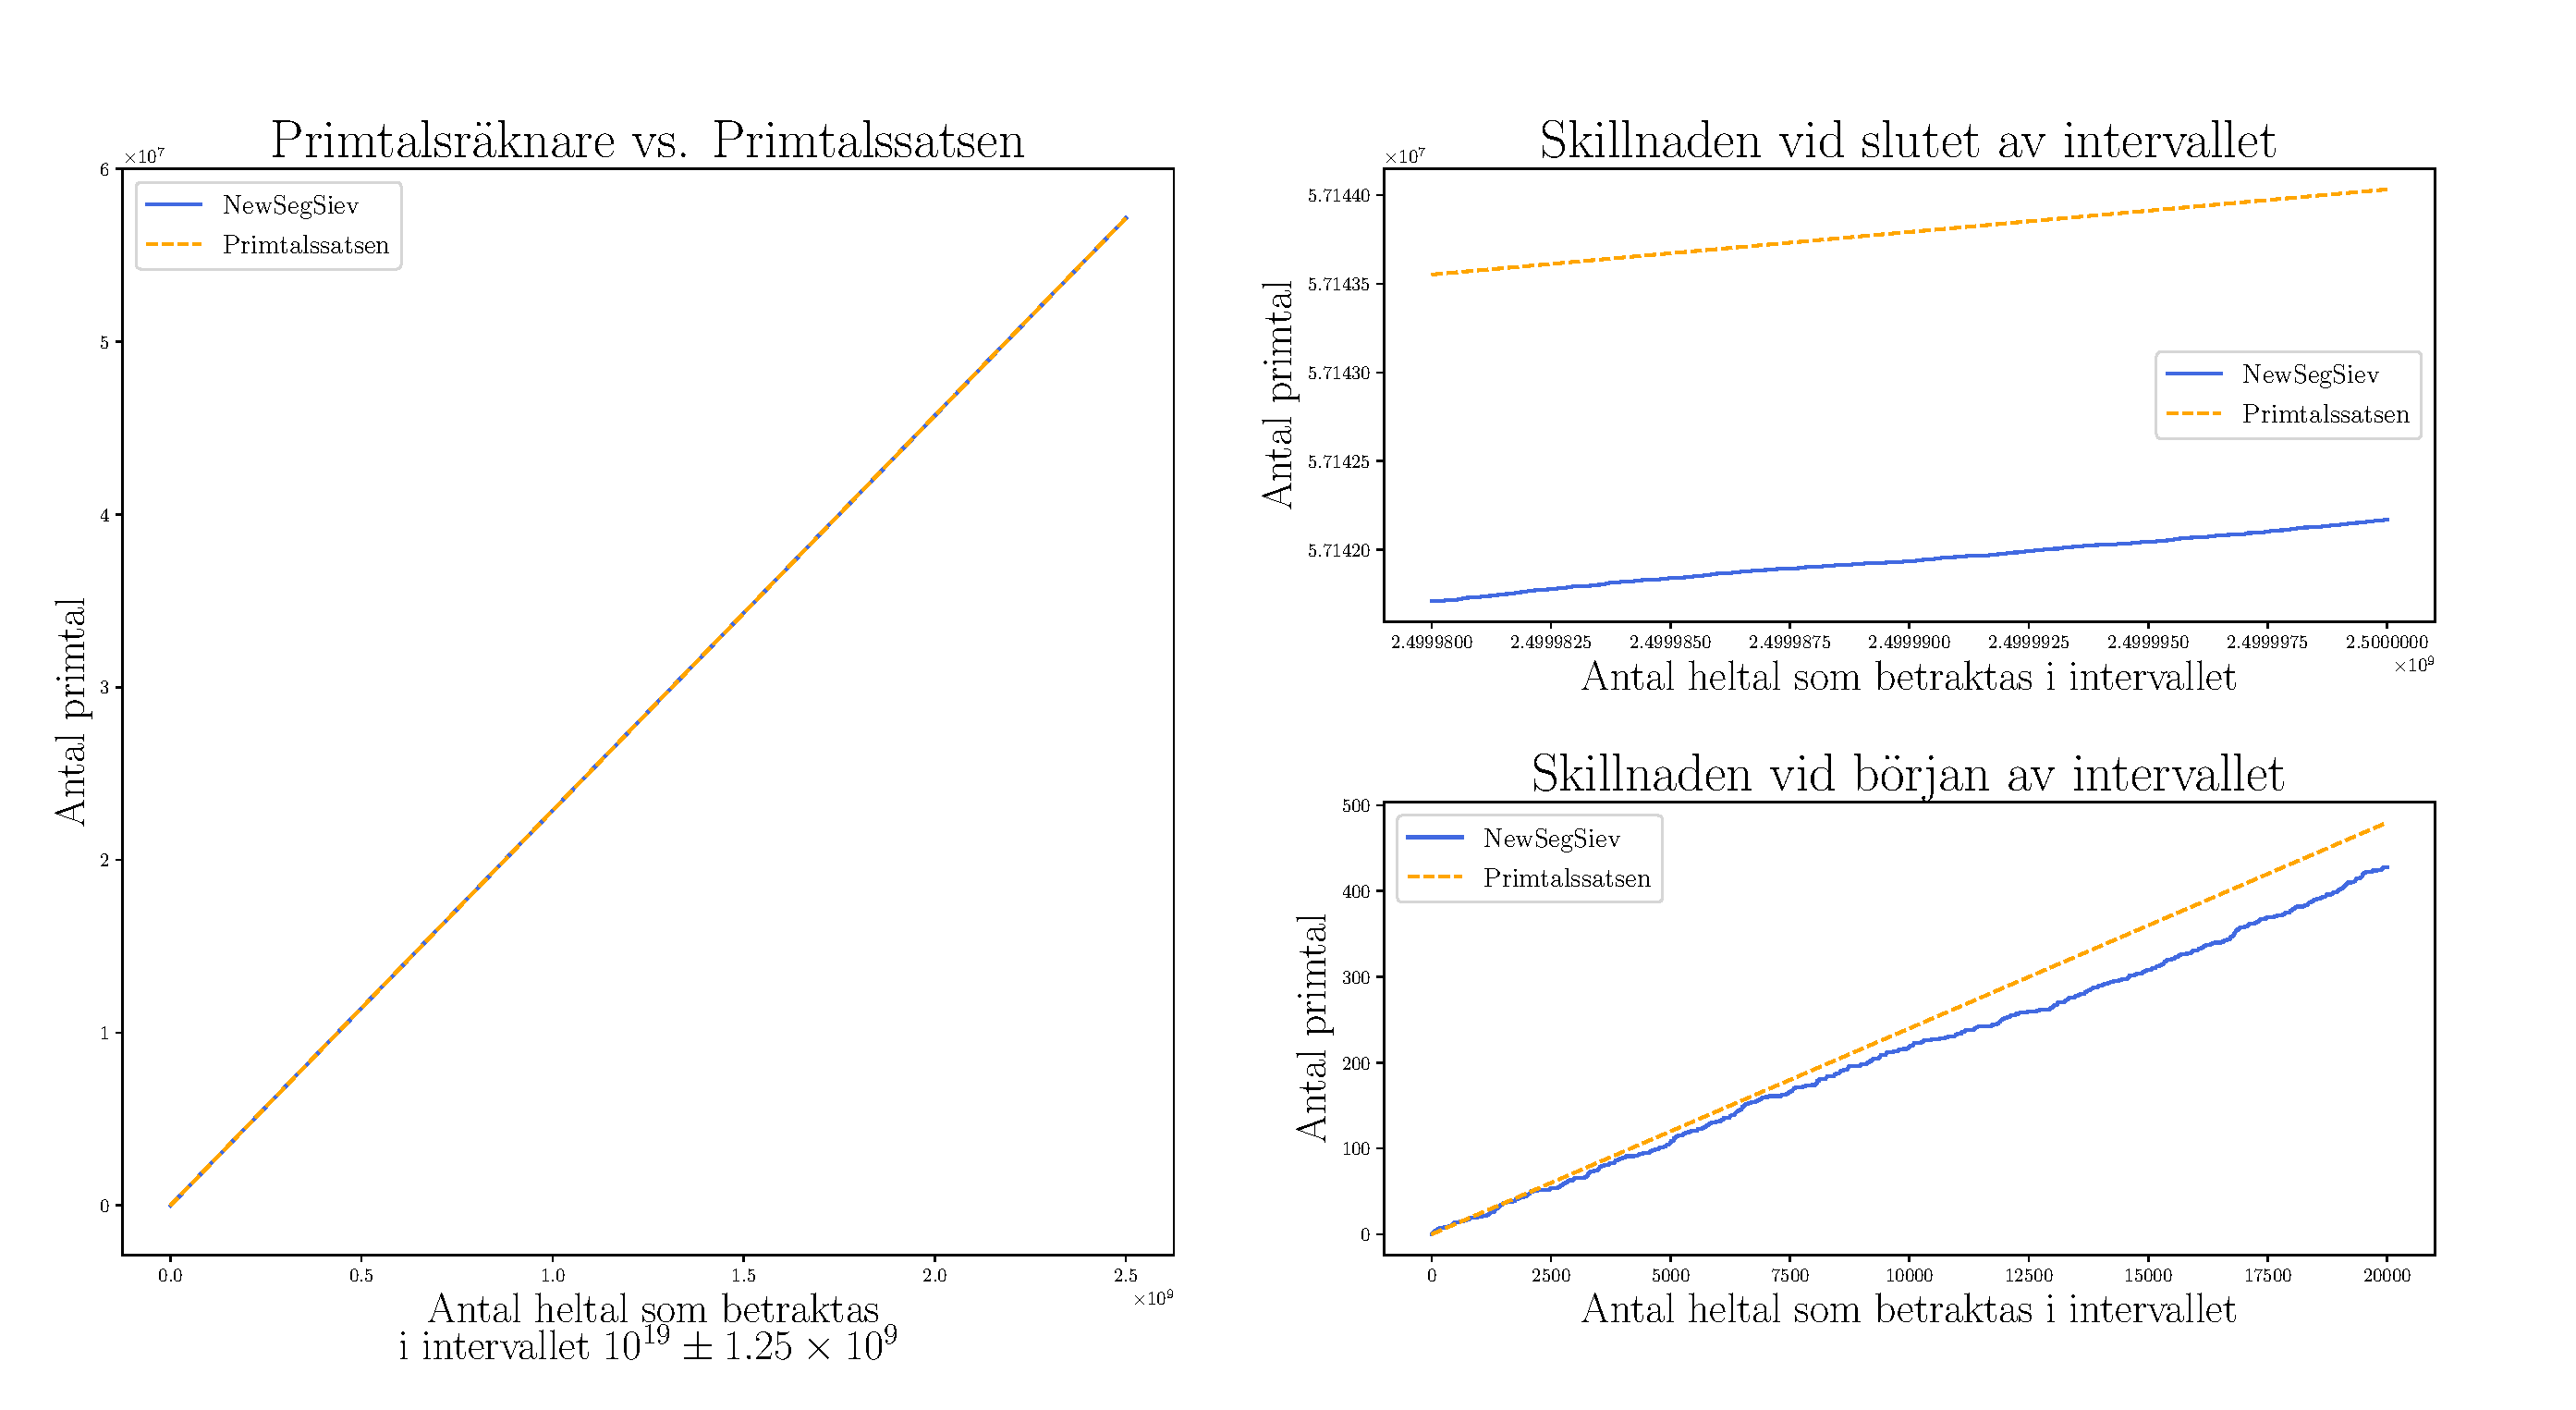
\includegraphics[width = \textwidth]{coen/Images/Primes.pdf}
    \caption{I figuren till vänster redovisas antalet primtal vilket förväntas enligt primtalssatsen, \textit{orange}, och antalet primtal som hittades enligt \textsc{NewSegSiev}, \textit{blå}, då \(n = 10^{19}\), \(\Delta = 1.25\cdot10^{9}\), och \(K = 2.5\). 
    Notera gärna att kurvorna ligger nästan på varandra. 
    I de figuren till höger redovisas en zoomad version av grafen till vänster för att visa skillnaden mellan vår uppskattning och det som förväntas vid mitten av intervallet, där algoritmen returnerar kring 1000 fler primtal än förväntat, och vid slutet av intervallet, där algoritmen returnerar kring 1700 färre.}
    %This graph shows the relative distributions of primees as per the aforementioned fucntions. Notice that while x over log x appears relatively close for smaller x the logarithmic integral approximation is a near exact match for the true distribution, so much so that the code line is hidden.
    \label{fig:res.prime}
\end{figure}
%As shown in figure X, should we believe in the PNT it seems as though our code does indeed find the correct number of primes. The rather large error in the x over log x estimate is indicative/reflective of one of the limitations highlighted in Section XXX, namely the impact of the error terms and their reconcillation with the main terms. Howeve, there doest exist a deeper link between the x over log x estimate and that of the logarithmic integral. Throguh the use of integral wizardry you can decompose the logarithmic integral into a series of terms, the first of which being x over log x with the remainder being of the order of sqrt(x). This then accounts for the increase in error as x grows. Thiese kinds of approximations for the prime counting function can also be rather naturally extrapolated to those for twin primes, as discussed below.

\todo{Diskussion needs work, going to be rewritten from scratch prolly}

Som vi ser i vänstra grafen av figur \ref{fig:res.prime}, då vi nu tror på primtalssatsen så verkar det som vår kod hittar det korrekta antalet primtal i intervallet, eftersom skillnaden mellan kurvorna är nästa osynlig på makronivå. 
Att de inte ligger exakt på varandra är en kombination av felet vilket inte visas i \eqref{app.primes.PNT}, felet skapat av interpoleringen som görs för att underlätta ritningen av graferna, och att egentligen är \(\pi(x)\) en stegfunktion. 
Vi väljer parametrarna som de är för att först undersöka långt ifrån noll, med tanke på att öka feltermen för \eqref{app.primes.PNT}, och därför valde så stort \textit{n}\footnote{Att \textit{n} inte valdes större i detta fallet är på grund av körningstiden för koden.}.
Följaktligen väljer vi \(\Delta\) på så sätt att vi använde Helfgotts förbättringar i \textsc{NewSegSiev}, \textsc{DiophAppr} funktionen, och för att göra det krävs en specifik storlek på intervallet.
Slutligen väljer vi \textit{K} till 2.5 för att det är minsta K:et som kan vals enligt Helfgott.
Tillsammans bildar dessa parametrar en bra bas för de följande tillämpningar då vi sparar bitarry:n och läser in den istället för att hitta alla primtal över igen.
\todo{Diskutera mer varför detta gör algoritmen pålitligt/kommentera på hur nogrannt Eratosthenes algoritm är}

\subsubsection{Fördelningen av tvillingsprimtal}
%Continuing our presentation of various sets of prime's distributions, next we turn to the other recurring theme of twin primes. The following figure illustrates the distributions of twin primes as predicted by x over log squared x and the second order logarithmic integral against those primes found using our implementation. It should be noted that a rather simple help function, Appendix XXX, was written which searches for non twin primes in the prime list and removes them.

Med hjälp av de primtal vi hittade i \ref{app.primes.title}, vänder vi oss nu till tvillingsprimtal och deras hypotetisk fördelning. Det finns ingen sats för tvillingsprimtal vilket motsvarar primtalssatsen för enkla primtals fördelning, dock så finns det en hypotetisk fördelning vilket är
\begin{equation}
    \pi_2(x) \sim 2C_2\cdot Li_2(x) = 2C_2\int_2^x\frac{1}{(\log t)^2}dt\label{app.twins.TWN}
\end{equation}
där \(C_2 = 0.6608...\) är tvillingsprimtalskonstanten. Genom att utveckla vår kod lite kan vi hitta alla tvillingsprimtal i de primtal vi har genererad och sedan jämföra vår fördelning emot den hypotetiska. Vi utveckla koden genom att introducera en funktion, Appendix XXX, vilket sållar bort alla icke tvillingsprimtal i en lista av primtal.

\begin{figure}[H]
    \centering
    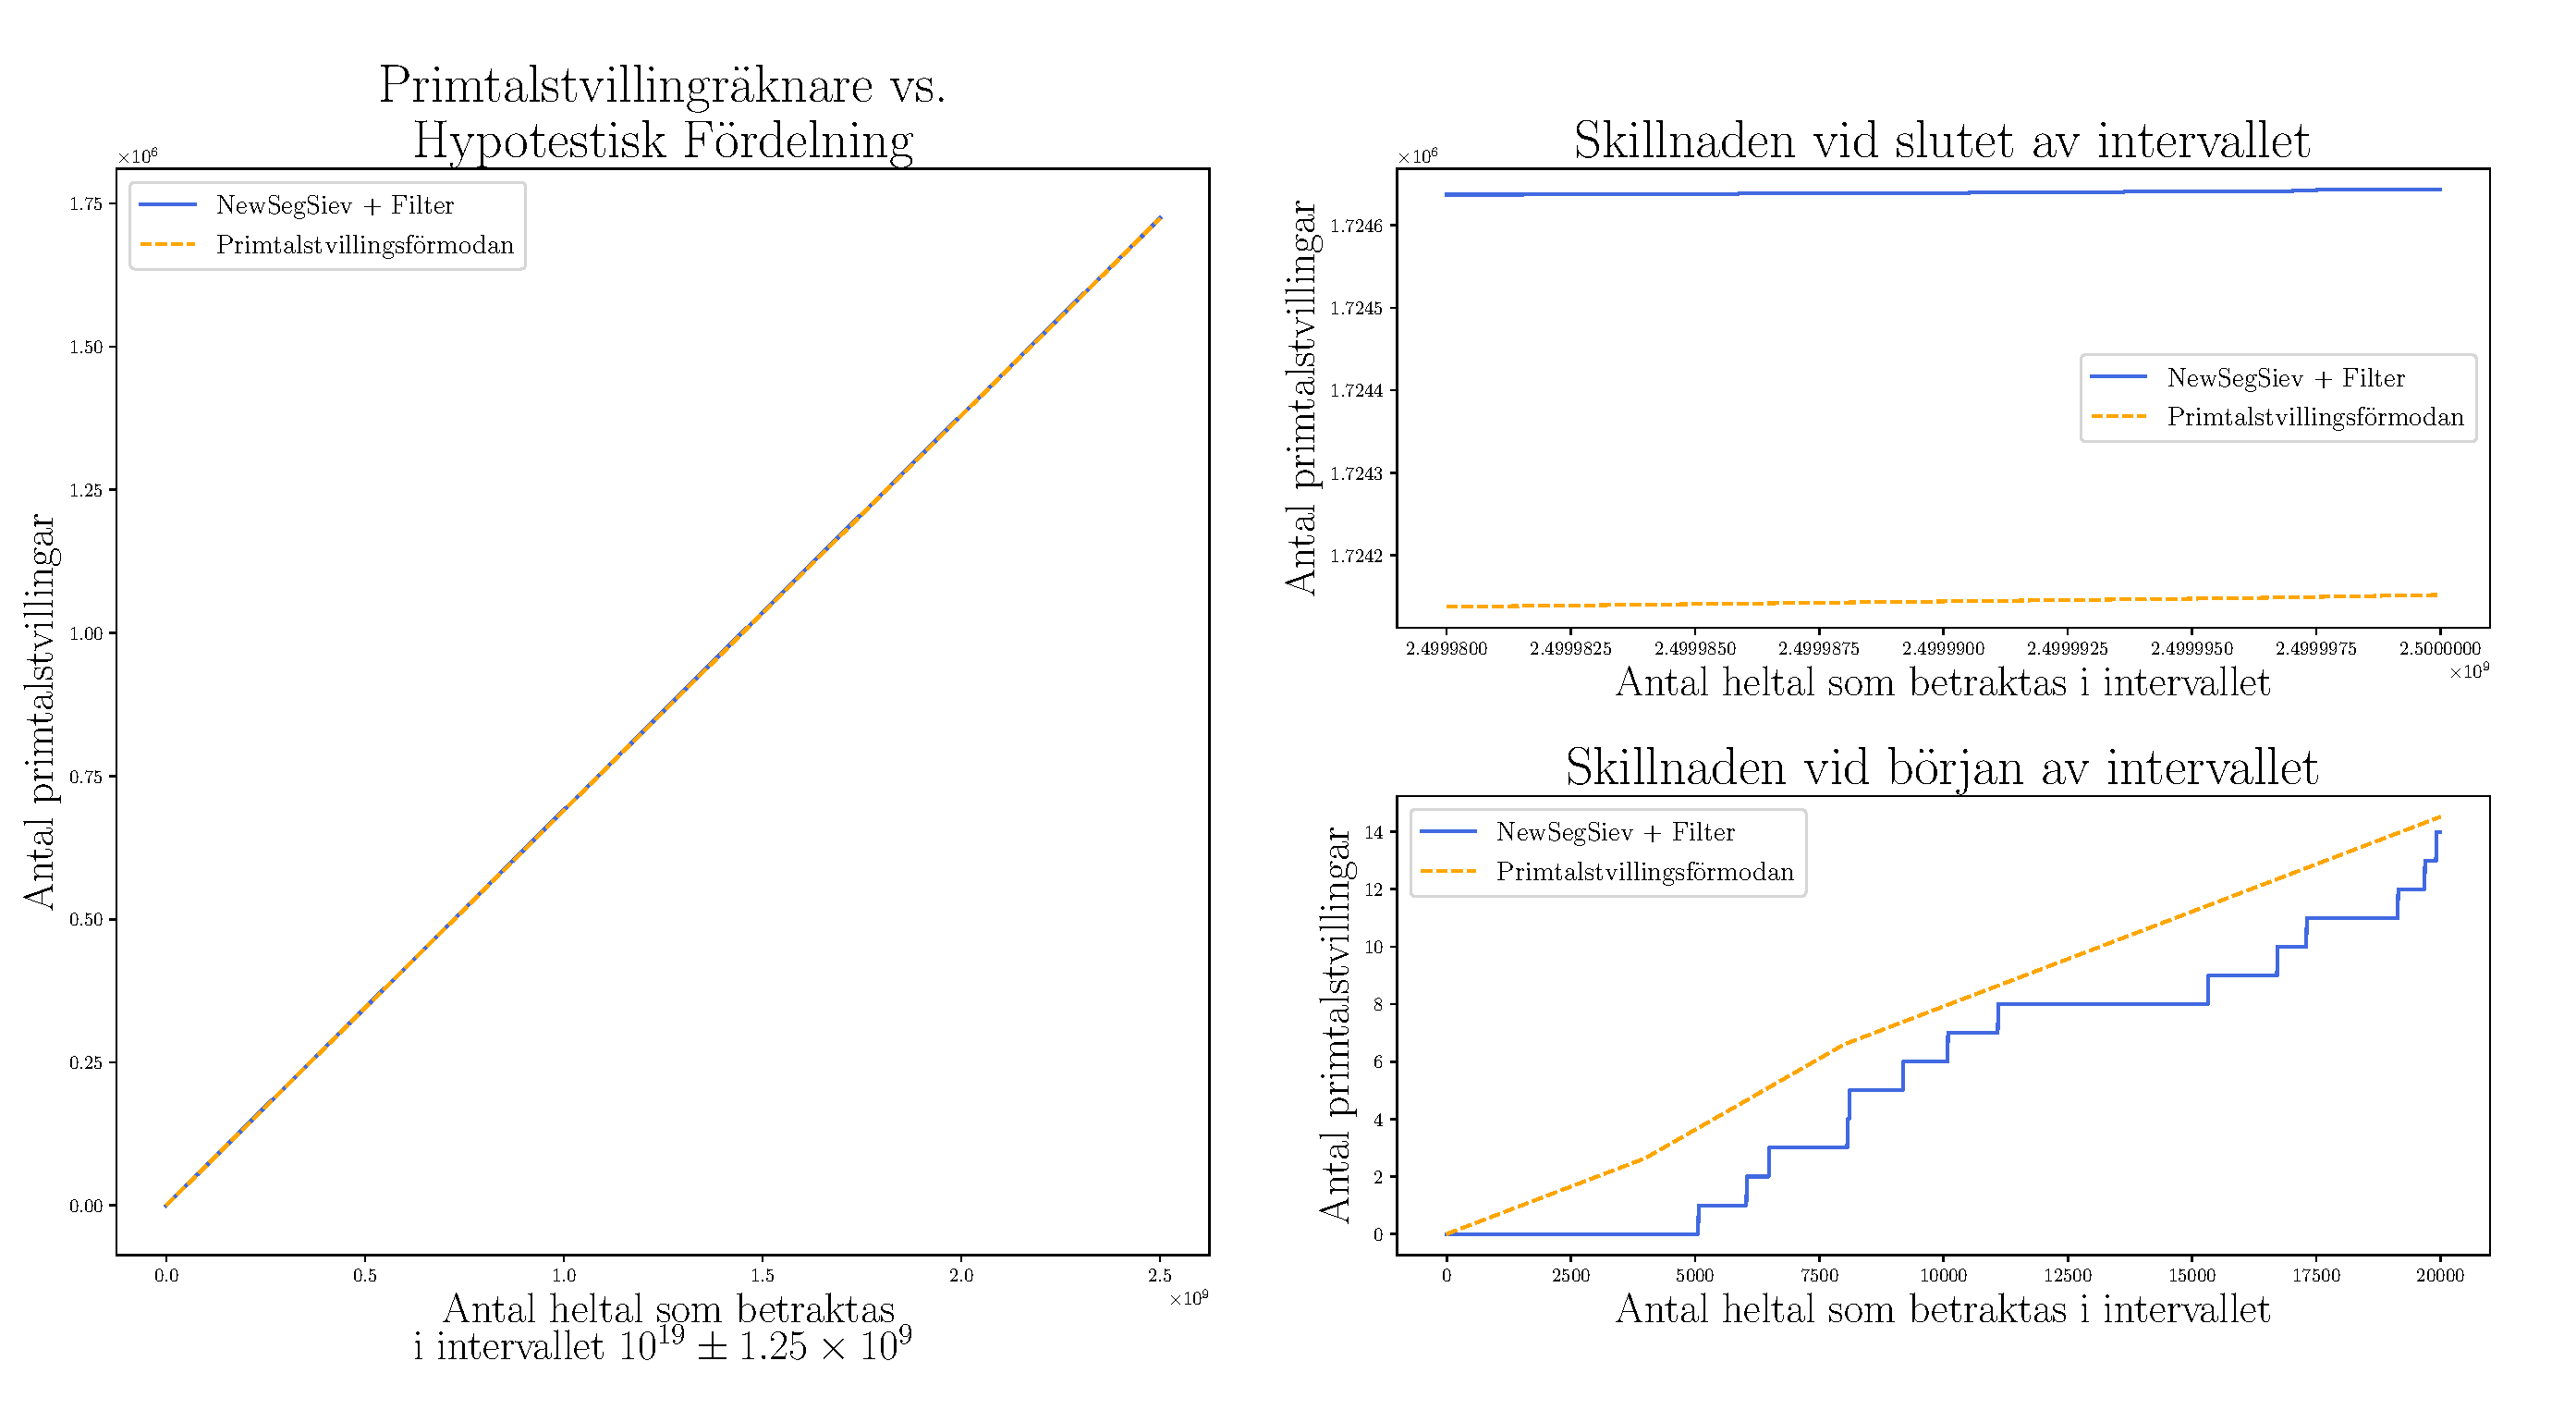
\includegraphics[width = \textwidth]{coen/Images/TwinPrimesNoKapp.pdf}
    \caption{\todo{Explanation of and commnents on graphs}}
    %This graph shows the relative distributions of the twin primes as per the aforementioned fucntions. Notice once again the accuarcy of the logarithmic integral, once again hiding our code line, as opposed to that of C x over log squared x, where the constant is 2*C_2, or 2 times the twin prime constant (discussed below).
    \label{fig:res.twins}
\end{figure}
\todo{Diskutera och förklara varför saker ser ut som de gör, vad detta säger för tvillingsprimtalshypoteseen och hur vår val av C2 har påverkat saker}
%There are a number of things to discuss regardng the above figure. 
\subsubsection{Frekvens av primtalsgapp}
\todo{Introducera de förändringarna som utfördes för att tillåta koden att bestämma storleken på primtalsgapp. Koppla till inledningen och vad detta har att göra med sållteori}
\begin{figure}[H]
    \centering
    
\includegraphics[width = 0.7\textwidth]{coen/Images/test.png}
    \caption{\todo{Infoga en histogram och sedan påpeka mönster}}
    \label{fig:res.arit}
\end{figure}
\todo{Diskutera ovanstående graf. Varför har vi vad vi har? Hur kan detta kopplas till tvillingsprimtal?}